Przed uruchomieniem i~przetestowaniem systemu, należy najpierw zainstalować wszystkie zależności i~uruchomić odpowiednie moduły.

\subsection{Instalacja i uruchomienie systemu}
W~celu uruchomienia obu usług, a~co za tym idzie całego systemu, należy w~pierwszej kolejności przygotować wirtualne środowisko Pythona. Wraz z~kodem źródłowym, dostarczone zostały dwa pliki \texttt{Pipfile} oraz \texttt{Pipfile.lock}. Opisują one wersję interpretera Pythona, a~także wszystkie potrzebne zależności, które muszą zostać zainstalowane przed uruchomieniem modułów. Dodatkowo, drugi plik opisuje dokładne wersje tych zależności. Dzięki zastosowaniu wirtualnego środowiska, eliminujemy problem różnych wersji zależności, już znajdujących się na maszynie docelowej. Aby utworzyć nowe środowisko, należy wykonać polecenia \texttt{pipenv~shell} oraz \texttt{pipenv~install}.

Dodatkowo, w~celu umożliwienia poprawnego działania modułu \texttt{Zapytajka}, należy zainstalować silnik przeglądarki Firefox. W~tym celu, należy wykonać polecenie \texttt{webdrivermanager firefox}.

W celu uruchomienia obu modułów, należy wykorzystać serwer wsgi \texttt{gunicorn}. Uruchomienie serwerów dzieje się przy użyciu następujących poleceń:
\begin{center}
    \texttt{gunicorn -w 4 kps:app}
\end{center}
oraz 
\begin{center}
    \texttt{gunicorn -w 4 summary\_{}search:app}
\end{center}

\subsection{Instrukcja użytkownika}
Aby skorzystać z~aplikacji klienckiej, należy uruchomić dowolną przeglądarkę oraz przejść pod adres \texttt{http://localhost:5000}. Uruchomi to stronę internetową z~prostym formularzem. Należy wybrać silnik wyszukiwania, strategię generowania zapytań i~wpisać pytanie. Po wypełnieniu formularza, należy go potwierdzić, klikając przycisk \textit{Zadaj}. Rozpocznie to proces wyszukiwania odpowiedzi. Po chwili, pojawi się kolejna strona ze znalezioną odpowiedzią oraz linkiem do dokumentu, w~którym można znaleźć więcej informacji.

\begin{figure}[h]
    \centering
    \fbox{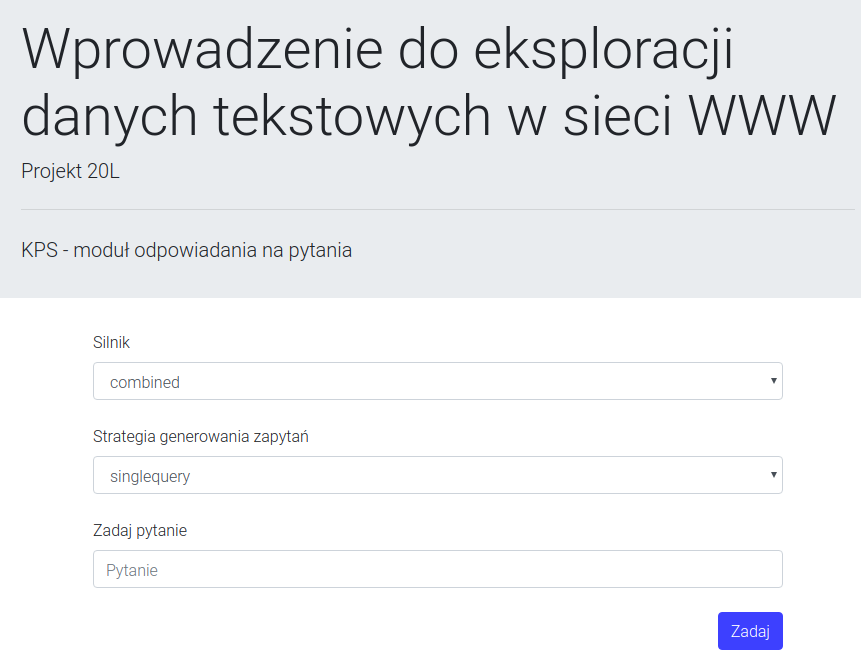
\includegraphics[width=\columnwidth]{figures/kps.png}}
    \caption{Formularz do zadawania pytań}
    \label{fig:algorithm-overview}
\end{figure}
